\documentclass[10pt,a4paper,twoside]{article}
\usepackage[dutch]{babel}
\usepackage[utf8]{inputenc}
\usepackage{amsmath}
\usepackage{graphicx}
\graphicspath{ {./dbms/} }
\usepackage{float,flafter}
\usepackage{hyperref}
\usepackage{inputenc}

\setlength\paperwidth{20.999cm}\setlength\paperheight{29.699cm}\setlength\voffset{-1in}\setlength\hoffset{-1in}\setlength\topmargin{1.499cm}\setlength\headheight{12pt}\setlength\headsep{0cm}\setlength\footskip{1.131cm}\setlength\textheight{25cm}\setlength\oddsidemargin{2.499cm}\setlength\textwidth{15.999cm}

\begin{document}

\begin{center}
\hrule

\vspace{.4cm}
{\bf {\Large TERM PAPER  }}\\
\vspace{.3cm}
{\bf {\huge Big data management challenges in healthcare }}
\vspace{.3cm}
\end{center}

{\bf Name:}  Priyanshu Gupta

{\bf Roll no:}  19111042 

{\bf Branch: } 6th Biomedical Engineering, 2022 
\\
\hrule

\vspace{.3cm}
\section*{Introduction} 
What is Big data?\\
Big Data is a term used for addressing a huge and heterogeneous amount of data too large to be handled with common software systems. The information contained by this data set can be classified into various groups and many dimensions. Such versatile databases are fragile enough and immense in volume requiring a powerful and dynamic management system including software, infrastructure to meet today’s demand and privacy plus security concerns. Besides these, management should be powerful enough to make it available in real time, which will allow it to be analysed and used immediately. \\
 
\textbf{Big data in healthcare}\\
A similar demand follows in the healthcare systems. At every level of medical care, the different kind of information either be it a patient’s medical history or a medical and clinical data, everything is equally informative for next surgery or appointment. Also it is a tedious job to maintain each and every hardcopy of a person’s medical history and present when ever needed. Due to this need, a new system Electronic health records (EHR) was introduced which represent records maintained electronically for improving the health care sector towards the benefit of patients and clinicians. In the era of telemedicine with so much advancement in computer systems, the digitalization of medicine along with medical records and all clinical test and experiment reports is becoming a standard. Nowadays, every single information is working through cloud and healthcare is becoming one such discipline. This information from clinical studies, research and observations of individuals’ lifestyle and environmental exposure are all of great value towards advanced health research, since they work as a training datasets for predictive models for the solution and ease of real life biomedical problems. The increasing availability of omics data from a single blood test to surgeries and research reports contributing to the Big data is becoming a major challenge across health research disciplines.    \\


\begin{center}
    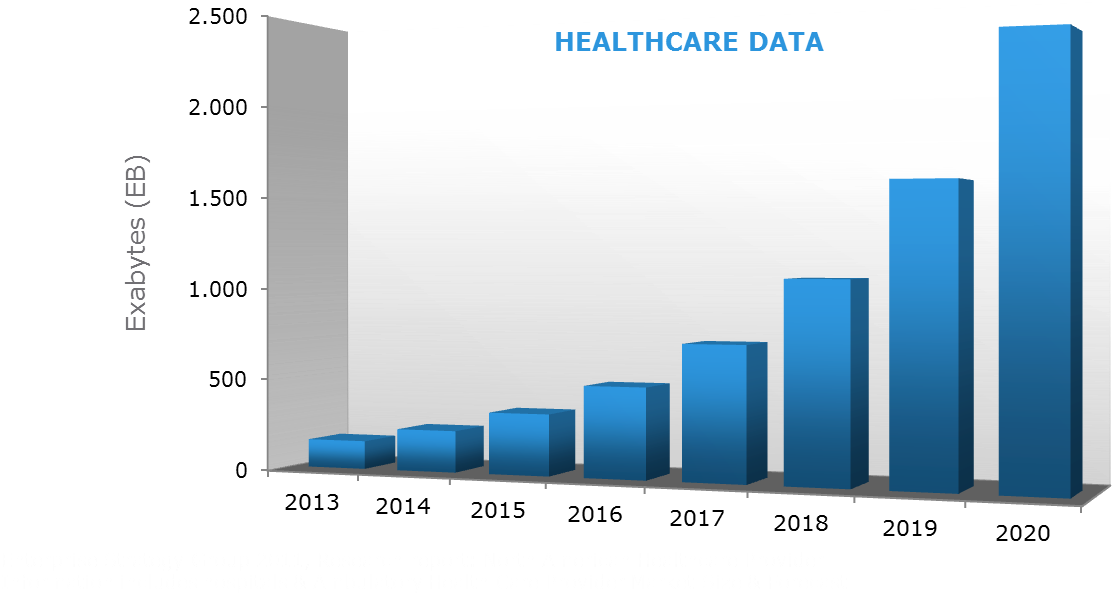
\includegraphics[width=15cm, height=8cm]{healthcaredata} \\[\baselineskip]
\end{center}

\section*{Challenges associated with healthcare big data }
\textbf{Current data management practice in health research }

The huge and heterogeneous big data in healthcare is less informative with normal database systems. The common software frameworks for operating big data analysis are high power computing clusters that are accessible via grid computing infrastructures. \textbf{Apache Hadoop} is an open source software framework for large-scale storing and processing of big data. Hadoop comprises of two components, Hadoop Distributed File system (HDFS) and MapReduce. The latter one is used to partition the input into smaller sub problems by a master process and then distribute it to worker processes. It was used in the bioinformatics field under the project on “The Cancer Genome Atlas”. The process of “sharding” i.e. splitting genome data into smaller more manageable chunks was carried out using the Hadoop framework together with the Genome Analysis Toolkit. Another framework based on Hadoop is the \textbf{Apache Hive}. It is a distributed data warehouse infrastructure that supports data summarization, query and analysis of large datasets stored in (HDFS).

\begin{center}
    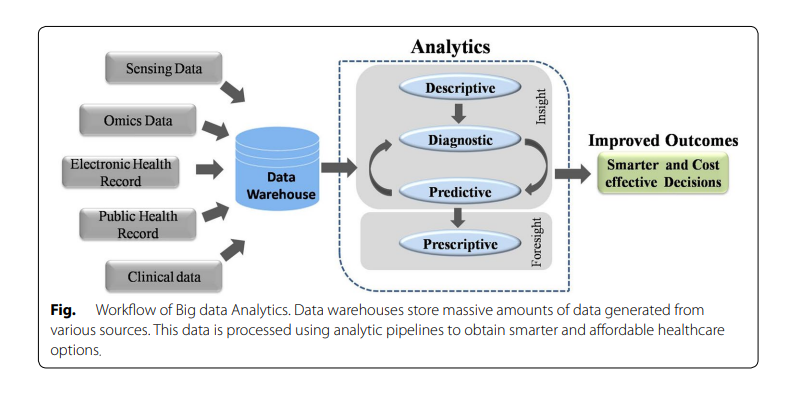
\includegraphics[width=16cm, height=9cm]{analytics} \\[\baselineskip]
\end{center}

For healthcare, the data gathered from various sources is mostly required for optimizing consumer services rather than consumer consumption. The heterogeneity, the noise and variety of the experimental techniques and the biological conditions these data should be considered, before integration in the database. Later on, different data mining techniques could be applied on these datasets such as: anomaly detection, clustering, classification, association rules summarization and visualization of these big data sets. These tools can help extract knowledge from patients’ care data to analysis and suggest innovative services to save their lives and to develop innovative techniques to diagnose and treat various diseases.
\\[\baselineskip]

\textbf{Data management approaches }\\
In biomedical data capture and archiving practice, both RDBMS and NoSQL DBMS have been used to build database tools.

\begin{itemize}
 \item \textbf{The relational database RDBMS:} This is often used for information integration or normalisation. The SQL approach can develop data structures with Atomicity, Consistency, Isolation and Durability (ACID). The database flexibility and scalability of the SQL approach rely on a clean separation between data structure and data values, as well as correct identification and construction of data relations and relationships. The final product of this process is an executable database schema, in which all the atomic data elements (i.e. attributes) are meant to be highly reusable so that the schema can be relatively stable and generalizable across studies. The relational database models (RDBMS) are not suitable for Big Data problems because they lack horizontal scalability and need hard consistency and become very complex when representing structured relationships.

 \item \textbf{The non-relational approaches: }This is for information centralisation. The NoSQL solutions focus on data availability, so they generally do not require rigorous data attribute atomicity (i.e. normalization) nor demand predefined data relationship. Therefore, these are often referred to as ‘open schema’ or ‘schema-flexible’. Even if the NoSQL approach has proven to be a potent solution for information centralization and target finding, especially in big data applications, the inability to query granular-level semi-structured or unstructured data is a common problem with NoSQL repositories in the biomedical data space. In that situation, users have to download the entire data set to figure out details on their own.
\end{itemize}

\section*{Big Data Challenges }
The main issue is the need of reliable system to deal with a dataset whose size is beyond the management capabilities of normal database software. And to make it available to the scientists for analysis, it should be stored in file format that would be easy to access and work on. For effective analysis, knowledge extraction of correct data is one of the many challenges. 

\begin{center}
    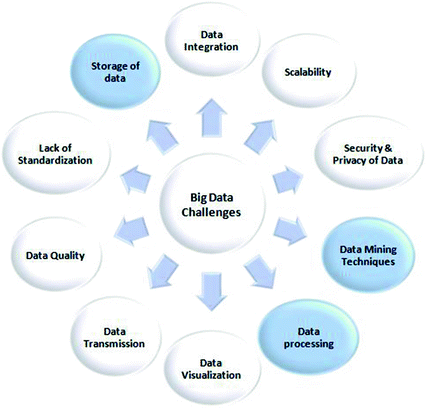
\includegraphics[width=12cm, height=11cm]{bdc} \\[\baselineskip]
\end{center}

Many Big Data management systems in the past have faced the V’s challenges namely volume, variety, velocity and veracity with the last V significant to health research.

\begin{enumerate}
    \item 	The volume demands versatile storage availability and accurate approaches for retrieval of information.
    \item	The variety allows for various combinations of grouping and different perspective for research.
    \item   The velocity or the accelerating rate of generation of data.
    \item	The veracity is the measurement of accuracy of the data organised.
\end{enumerate}

Storage only represents one face of the problems. The data-sets created without comparability and communicability is itself a layer of data heterogeneity. The real goal is to change the heterogeneous data into usable information and real knowledge. The Biological information is very rare and complex and so would be the algorithms involved in analysing them. \\[\baselineskip]

\section*{Weak sides of Big Data in healthcare} 

\begin{center}
    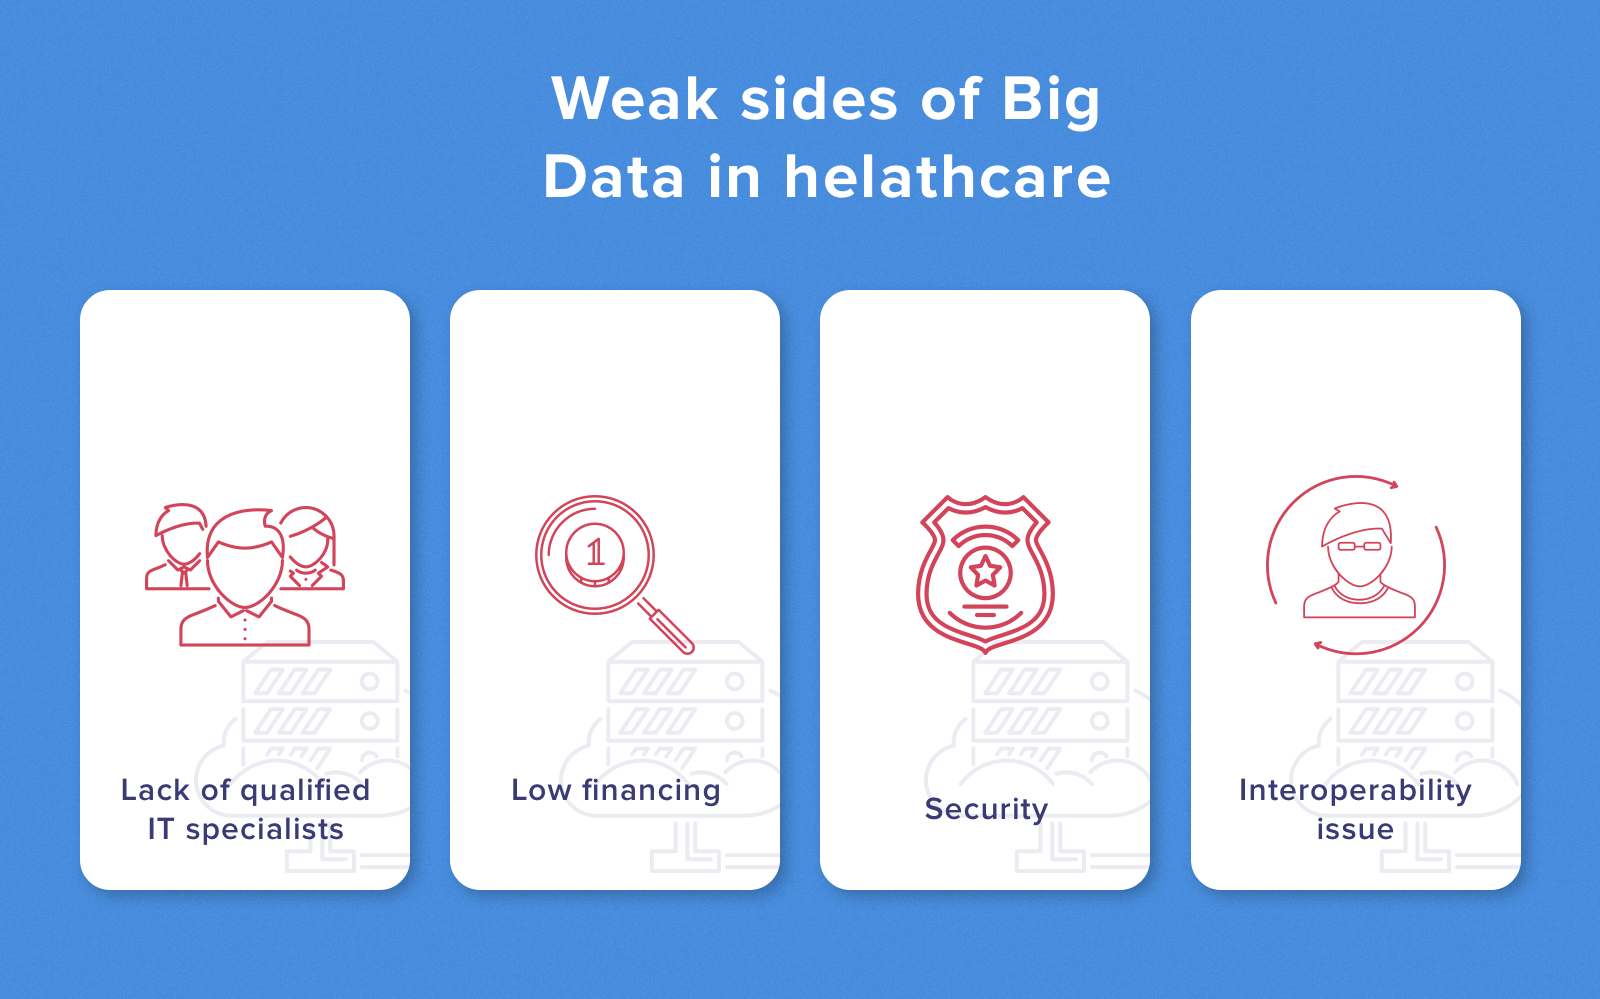
\includegraphics[width=14cm, height=9cm]{weak-sides} \\[\baselineskip]
\end{center}


\subsubsection*{Lack of qualified IT specialists }
Humans have a high scope of mistakes which can be entering missing values, incorrect data, misunderstanding or wrong interpretation of the original data. The EHRs data can be are very much influenced by the staff that entered the patient’s data. There are also not many IT specialists in the healthcare sector that can continuously manage and support the software and the clinics. Considering big data trends in healthcare, the necessity of skilled and talented IT staff cannot be neglected. They are the significant basic unit in digitalisation in healthcare.   


\subsubsection*{Low financing and Out-dated technology }
This is one of the biggest challenges since the medical department itself sometimes is not able to fulfil their needs with the funds provided. Therefore the digitalisation and big data department remains neglected and, research on leveraging cutting-edge methods and technologies to maximize the value of big data in health research remains underdeveloped. While purchasing a brand new server can be tough on budget, it’s easier than dealing with the fallout of a data breach.

\subsubsection*{Security and Privacy }
A network between multiple sectors and department sharing a large quantity of medical data creates a tempting opportunity for data thieves. In old days, when has to break into the hospital and physically search through files to access a person’s medical history. But now everything has changed drastically, all you need is some knowledge of hacking and a lack of moral balance in your thoughts. The fact is that if hospitals grant access to a few specialists then it is not a problem but if more people have access, it may lead to increased risk of privacy breach.  \\

Healthcare organizations must appoint good Big Data vendors having secure and advanced encryption algorithms and capable of pseudo-anonymisation of the personal data. These software solutions should provide security and authentication for all involved users, prevent all EHRs from the reach of third party applications as well as set up good governance standards and practices.

\pagebreak

\subsubsection*{Challenge of inter-operability}
Due to some reasons, many healthcare systems still cannot work together. 
Some reasons include the following ones: 

\begin{itemize}
    \item No specific healthcare protocols and standards 
    \item Discrepancies in privacy laws and chances of security breach when exchanging personal medical information 
    \item Old school approach i.e. still using paper health records 
    \item Difference in the use of terminology that can lead to incompatibility between two systems
\end{itemize}

\section*{Solutions}

\subsubsection*{Storage}
The cloud-based storage using IT infrastructure is becoming a better option having reliable costs and better understanding of the importance of healthcare-specific compliance and security issues. Besides, cloud storage offers lower up-front costs, nimble disaster recovery, and easier expansion.

\subsubsection*{Cleaning}
The data cleansing is important to ensure the accuracy, correctness, consistency, relevancy, and purity after acquisition. This process can be manual or automatized using logic rules and machine-learning techniques to ensure high levels of accuracy and integrity. For example, records no longer needed can be released to free up space and maintain consistency. It is too difficult to handle big data especially when it comes without a perfect data organization to the healthcare providers.\\

Medical coding systems like Current Procedural Terminology (CPT) must be developed and adopted to ensure the perfect data organisation and representation of core clinical concepts.

\subsubsection*{Accuracy}
The reporting of patient data into EHRs is not entirely accurate yet, probably because of poor EHR utility and complex workflows. The EHRs are intended to improve the quality and communication of data in clinical workflows. To achieve this, the quality improvement can be done by using self-report questionnaires from patients for their symptoms.

\subsubsection*{Image pre-processing}
The digitalisation and big data will help maintain the quality of image records and immune those from noise and artifacts. Medical images often suffer physical factors due to improper handling that can lead to altered data quality and misinterpretations from existing medical records.

\subsubsection*{Security}
A list of rules termed as HIPAA Security Rules can help protect health information. These can guide organizations with storing, transmission, authentication protocols, and controls over access, integrity, and auditing. Common security measures like using up-to-date antivirus software, firewalls, encrypting sensitive data, and multi-factor authentication can also prove to be beneficial.


\subsubsection*{Meta data}
The metadata compose of information like time of creation, purpose and person responsible for the data and also keep record of usage for researchers and data analysts. It would be mandatory to have complete, accurate, and up-to-date metadata regarding all the stored data as it increases the usefulness of data.

\section*{Discussions and Future Work}
High dimensionality of the – omics data means, that there have many more dimensions or features than the number of samples, and on the other side the EHRs data which regard to the individuals/patients, makes data mining techniques to be more challenging task. Keeping track of development in big data, the attempt to combine EAV with relational data tables in a RDBMS environment for biomedical data application reflects a clear desire and demand for the coexistence of SQL and NoSQL mechanisms in a single technology platform.\\

As a further work, these applications should enable applying data mining techniques to the heterogeneous and complex data to reveal hidden patterns and novel knowledge from the data. This novel knowledge should results with improving of the implemented healthcare to the patients as well to advanced decision making by the healthcare decision policy makers. It is therefore clear that in the Big Data field there is much to do in terms of making these technologies efficient and easy-to-use, especially considering that even small and medium size laboratories are going to use them in a close future.

\section*{References}

\begin{enumerate}
    \item https://www.sciencedirect.com/science/article/abs/pii/S0957417420302128
    \item https://www.degruyter.com/document/doi/10.1515/jib-2017-0030/html?lang=de
    \item https://pubmed.ncbi.nlm.nih.gov/28679881/
    \item https://journalofbigdata.springeropen.com/track/pdf/10.1186/s40537-019-0217-0.pdf
    \item https://sciendo.com/article/10.2478/dim-2018-0014
    \item https://www.virtru.com/blog/5-biggest-challenges-facing-healthcare-data-security-today/
\end{enumerate}


\end{document}

















